\documentclass[a4paper,11pt]{article}
\usepackage[utf8]{inputenc}
\usepackage[spanish]{babel}
\usepackage[margin=3.cm]{geometry}
\usepackage{amsmath,amsfonts,amssymb,amsthm,array}
\usepackage[all]{tcolorbox}
\usepackage{minted}
\usepackage{graphicx}
\usepackage{fancyhdr}
\usepackage{float}
\usepackage{multicol}
\usepackage{enumerate}

\newcommand\tab[1][1cm]{\hspace*{#1}}
\setlength{\headheight}{14pt}

\begin{document}
    \title{COMPUTACIÓN CONCURRENTE \\ {\Large EXAMEN 3: Algoritmos sin bloqueo y Consenso}}
    \author{
    	Prof. Manuel Alcántara Juárez \\
    	\texttt{manuelalcantara52@ciencias.unam.mx}
    }
    \date{Fecha: 2 de Febrero de 2021}

	\maketitle
	\pagestyle{fancy}

	\fancyhf{}
	\fancyhead[l]{Examen 3 - Oscar Andres Rosas Hernandez}
	\fancyhead[r]{Computación Concurrente}
	\fancyfoot[c]{\thepage}

\begin{enumerate}

    \item{Considerando la siguiente historia $H$:
    \begin{verbatim}
<A, q.enq(5)>
<B, p.enq(3)>
<B, p:void>
<B, p.enq(4)>
<A, q:void>
<C, q.deq()>
<B, p:void>
<C, q:5>
<A, p.deq()>
<B, q.enq(8)>
<A, p:3>
<A, q.enq(7)>
<C, p:deq()>
<B, q:void>
<C, p:4>
<B, q.deq()>
<B, q:8>
    \end{verbatim}
    \begin{enumerate}
        \item{
          \textbf{[0.5pt]} Dibuja el diagrama que representa la ejecución asociada.
          \begin{figure}[!h]
            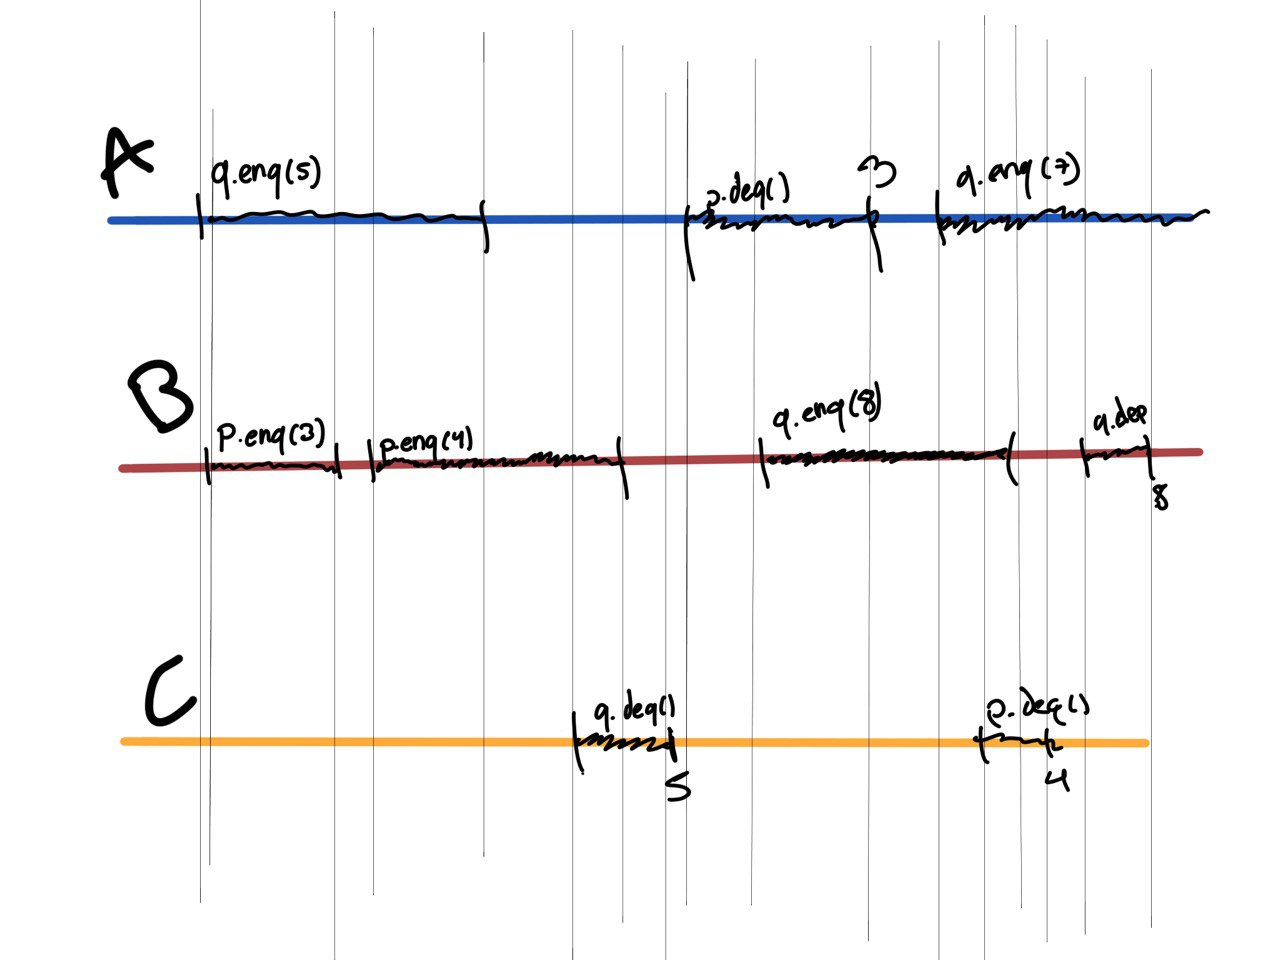
\includegraphics[width=\textwidth]{Graphics/1}
          \end{figure}

          \clearpage
        
        }
        \item{
          \textbf{[0.5pt]} Marca los espacios de quietud, 
          así como los puntos de linearización.

          \begin{figure}[!h]
            \centering
            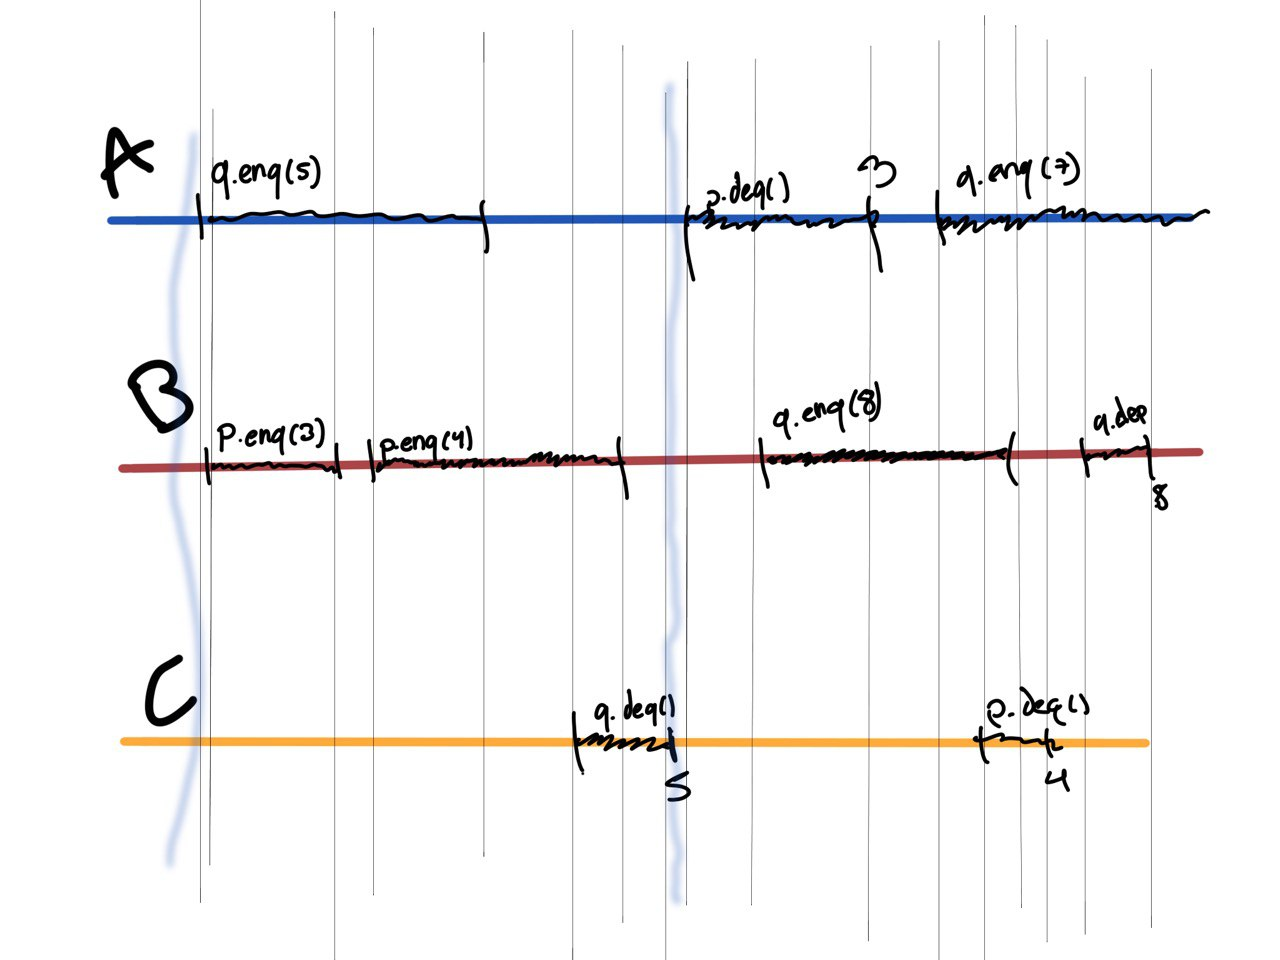
\includegraphics[width=0.3\textwidth]{Graphics/1a}
          \end{figure}

          }
        \item{
            \textbf{[0.5pt]} ?`Qué es $H|B$?

            Es el subconjunto de H, o subhistoria de H que solo incluye a los eventos de B, en este caso sería:
            \begin{verbatim}
              <B, p.enq(3)>
              <B, p:void>
              <B, p.enq(4)>
              <B, p:void>
              <B, q.enq(8)>
              <B, q:void>
              <B, q.deq()>
              <B, q:8>
            \end{verbatim}
            
            }
        \item{\textbf{[0.5pt]} ?`Que instrucción agregarías o quitarías para que $H$ sea completa?
            La forma mas facil es simplemente quitar la ultima instrucción de A, es decir dejar:

            \begin{verbatim}
              <A, q.enq(5)>
              <B, p.enq(3)>
              <B, p:void>
              <B, p.enq(4)>
              <A, q:void>
              <C, q.deq()>
              <B, p:void>
              <C, q:5>
              <A, p.deq()>
              <B, q.enq(8)>
              <A, p:3>
              <C, p:deq()>
              <B, q:void>
              <C, p:4>
              <B, q.deq()>
              <B, q:8>
            \end{verbatim}

            Pero tambien perfectamente puede agregar al final esto:
            \begin{verbatim}
              <A, q.enq(5)>
              <B, p.enq(3)>
              <B, p:void>
              <B, p.enq(4)>
              <A, q:void>
              <C, q.deq()>
              <B, p:void>
              <C, q:5>
              <A, p.deq()>
              <B, q.enq(8)>
              <A, p:3>
              <A, q.enq(7)>
              <C, p:deq()>
              <B, q:void>
              <C, p:4>
              <B, q.deq()>
              <B, q:8>
              <A, q:void>
              \end{verbatim}
        }
        

        \item{
          \textbf{[0.5pt]} ?`Es $H$ bien formada? ?`Porqué?
          
          Que H este bien formada quiere decir que todos las subhistorias, en este caso ($H|A$, $H|B$, $H|C$), son
          secuenciales.
          Y es cierto:

          \begin{verbatim}
            <A, q.enq(5)>
            <A, q:void>
            <A, p.deq()>
            <A, p:3>
            <A, q.enq(7)>
          \end{verbatim}

          \begin{verbatim}
            <B, p.enq(3)>
            <B, p:void>
            <B, p.enq(4)>
            <B, p:void>
            <B, q.enq(8)>
            <B, q:void>
            <B, q.deq()>
            <B, q:8>
          \end{verbatim}

          \begin{verbatim}
            <C, q.deq()>
            <C, q:5>
            <C, p:deq()>
            <C, p:4>
          \end{verbatim}

          }
        \item{\textbf{[1.0pt]} Indica todas las relaciones de precedencia en $H$.
        
          Facil de hacerse pero muy tardado de escribir, no me dio tiempo de hacerlo, perdon :c

        }
        
        \item{
          
        \textbf{[2.0pt]} Construye una historia legal y secuencial S equivalente a $H$. Argumenta porqué es legal y equivalente.
        Esta esta compleja de explicar de manera formal porque es equivalente y legal, es trivial demostrar
        que es secuencial, pues despues de cada invocacion lo que sigue es justo el retorno, 
        ahora podemos decir que es una historial legal porque no estamos moviendo de lugar los eventos,
        es 
        podemos demostrar que son equivalente pues no $S|A = H|A$ y $S|B = H|B$ y $S|C = H|C$.

        \begin{verbatim}
          <A, q.enq(5)>
          <A, q:void>
          <B, p.enq(3)>
          <B, p:void>
          <C, q.deq()>
          <C, q:5>
          <B, p.enq(4)>
          <B, p:void>
          <A, p.deq()>
          <A, p:3>
          <B, q.enq(8)>
          <B, q:void>
          <C, p:deq()>
          <C, p:4>
          <B, q.deq()>
          <B, q:8>
          <A, q.enq(7)>
        \end{verbatim}

        }
    \end{enumerate}
    }

    

      \clearpage

      \item{\textbf{[1.5pt]} Para cada una de las siguientes historias, menciona si son 
      secuencialmente consistentes, tienen la propiedad de consistencia de quietud
       o son linearizables. Justifica tu respuesta.
    \begin{enumerate}
        \item {
            \begin{verbatim}
<A, q.enq(x)>
<B, q.enq(y)>
<A, q:void>
<B, q:void>
<B, q.deq()>
<A, q.deq()>
<B, q:x>
            \end{verbatim}

              \begin{figure}[!h]
                \centering
                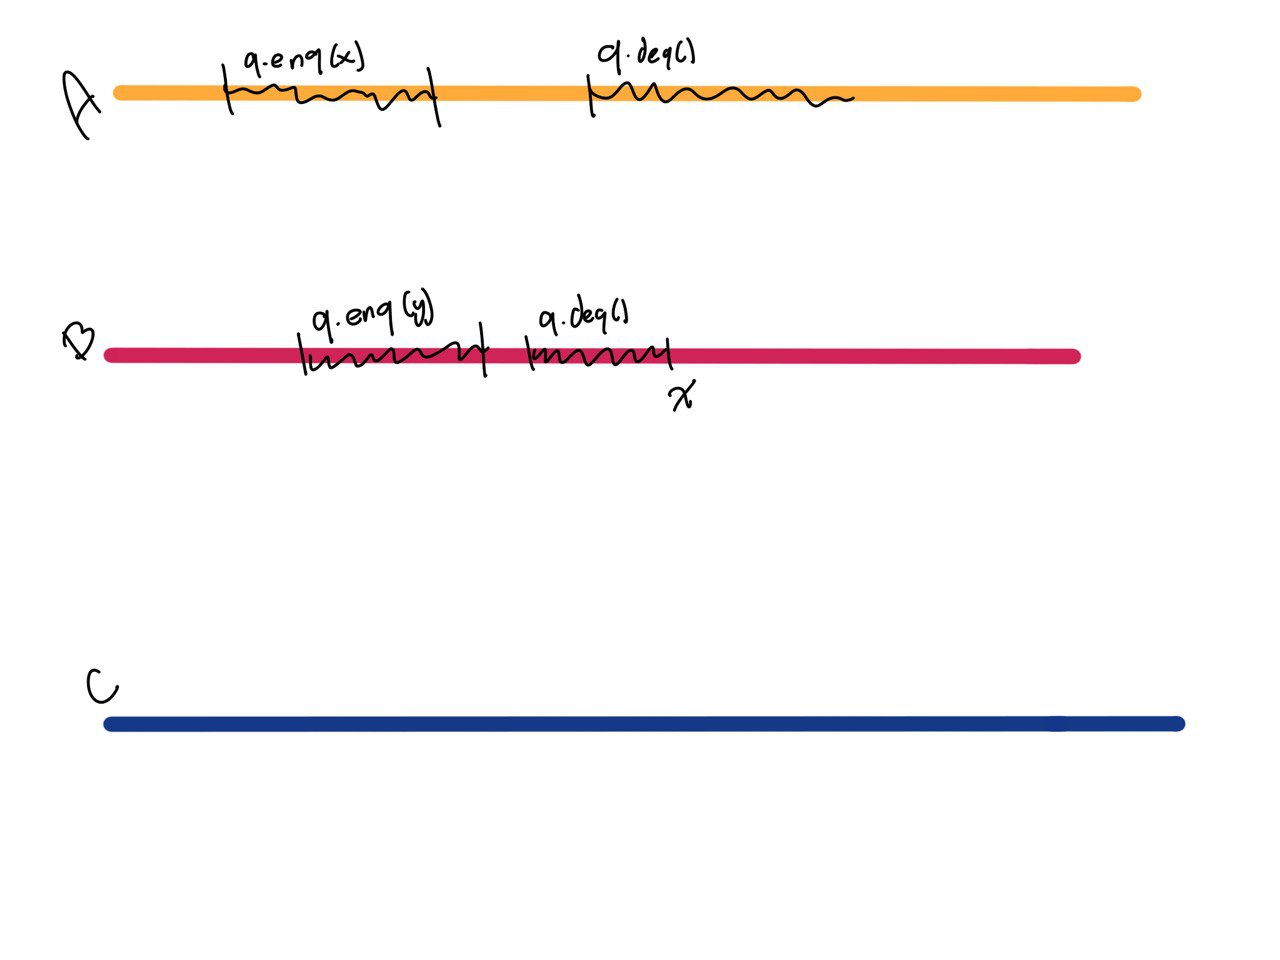
\includegraphics[width=0.3\textwidth]{Graphics/a}
                \caption{El diagrama sería}
              \end{figure}
  
              
              \begin{figure}[!h]
                \centering
                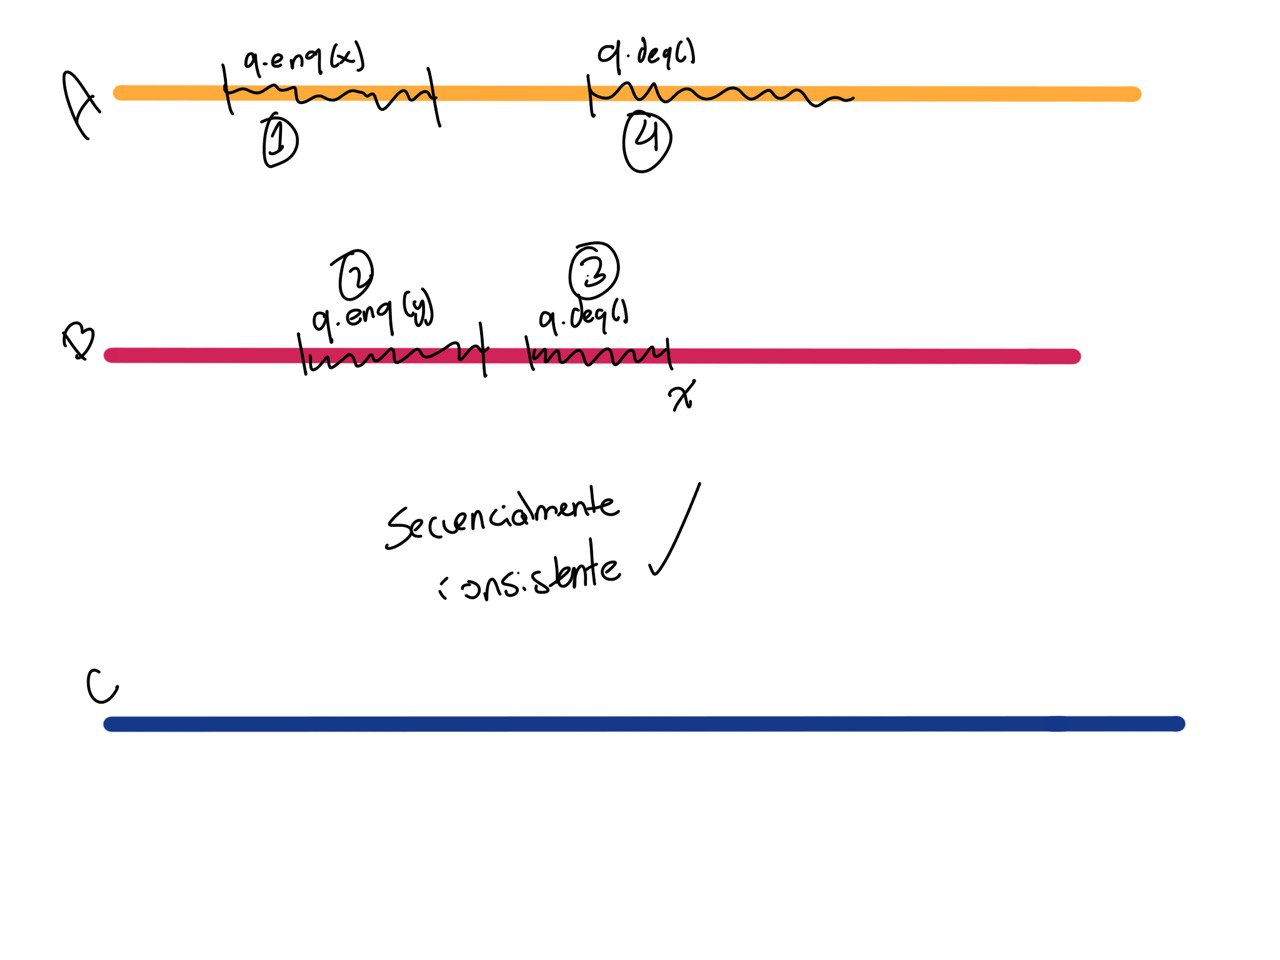
\includegraphics[width=0.3\textwidth]{Graphics/a_s}
                \caption{Secuencialmente consistente, pues podemos darle un orden a los eventos
                tal que el orden de los eventos dentro de cada hilo se mantiene y el orden
                resultante tiene sentido. }
              \end{figure}
  
              
              \begin{figure}[!h]
                \centering
                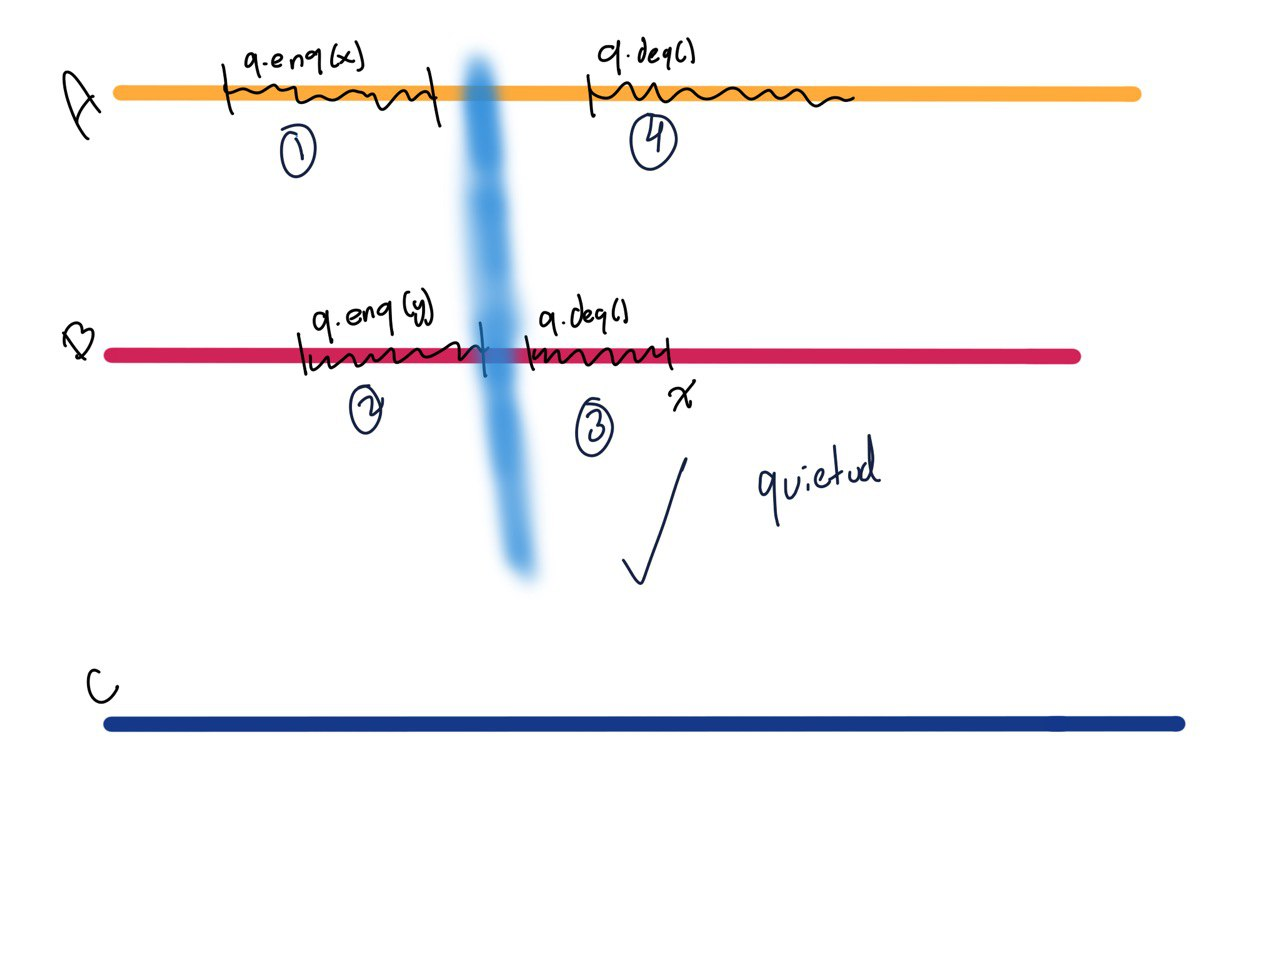
\includegraphics[width=0.3\textwidth]{Graphics/a_q}
                \caption{Consistencia de quietud, pues solo existe un espacio de quietud, y podemos
                dar un orden, el que mostramos por ejemplo, donde se respeta el orden de los eventos
                por bloques de quietud y el orden resultante tiene sentido. }
              \end{figure}
  
              \begin{figure}[!h]
                \centering
                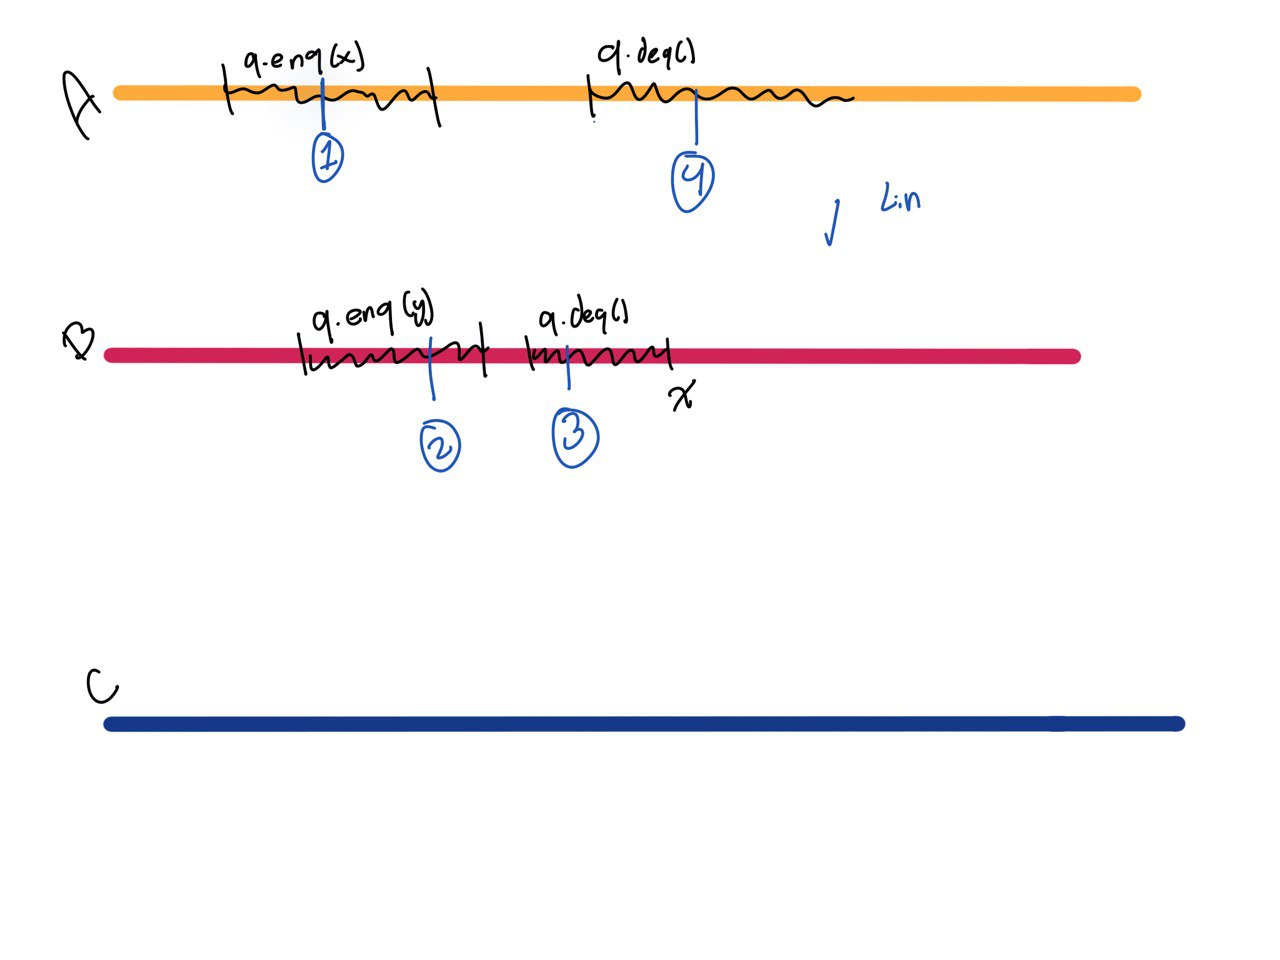
\includegraphics[width=0.3\textwidth]{Graphics/a_l}
                \caption{Linearizable, pues podemos dar un tiempo puntual para cada evento y con ello
                un orden resultante que tiene sentido. }
              \end{figure}
        }

        \clearpage

        \item 
        {
            \begin{verbatim}
<A, q.enq(x)>
<B, q.enq(y)>
<A, q:void>
<B, q:void>
<A, q.deq()>
<C, q.deq()>
<A, q:y>
<C, q:y>
            \end{verbatim}

            \begin{figure}[!h]
              \centering
              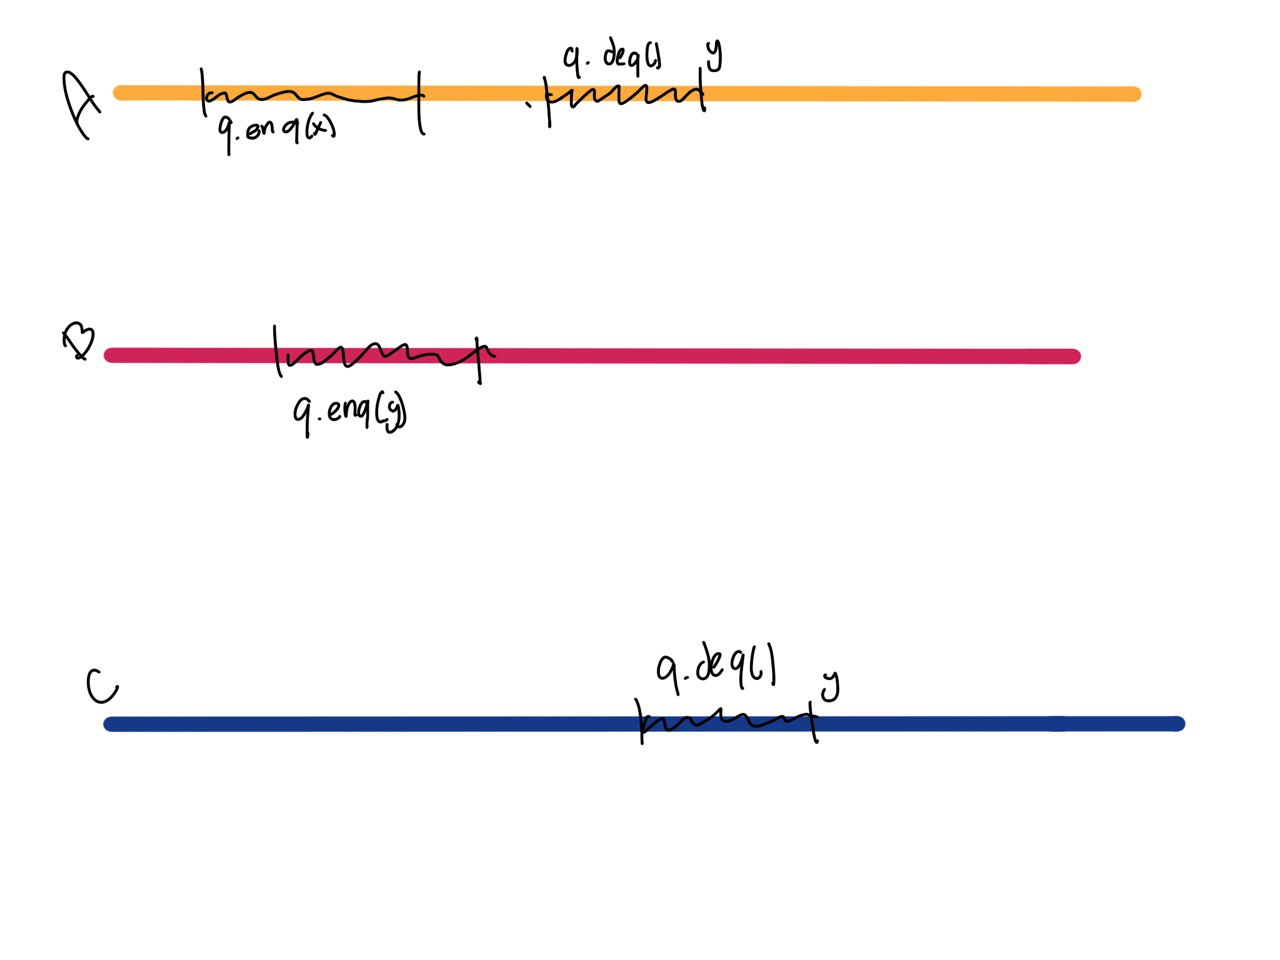
\includegraphics[width=0.3\textwidth]{Graphics/b}
              \caption{El diagrama sería}
            \end{figure}

            
            \begin{figure}[!h]
              \centering
              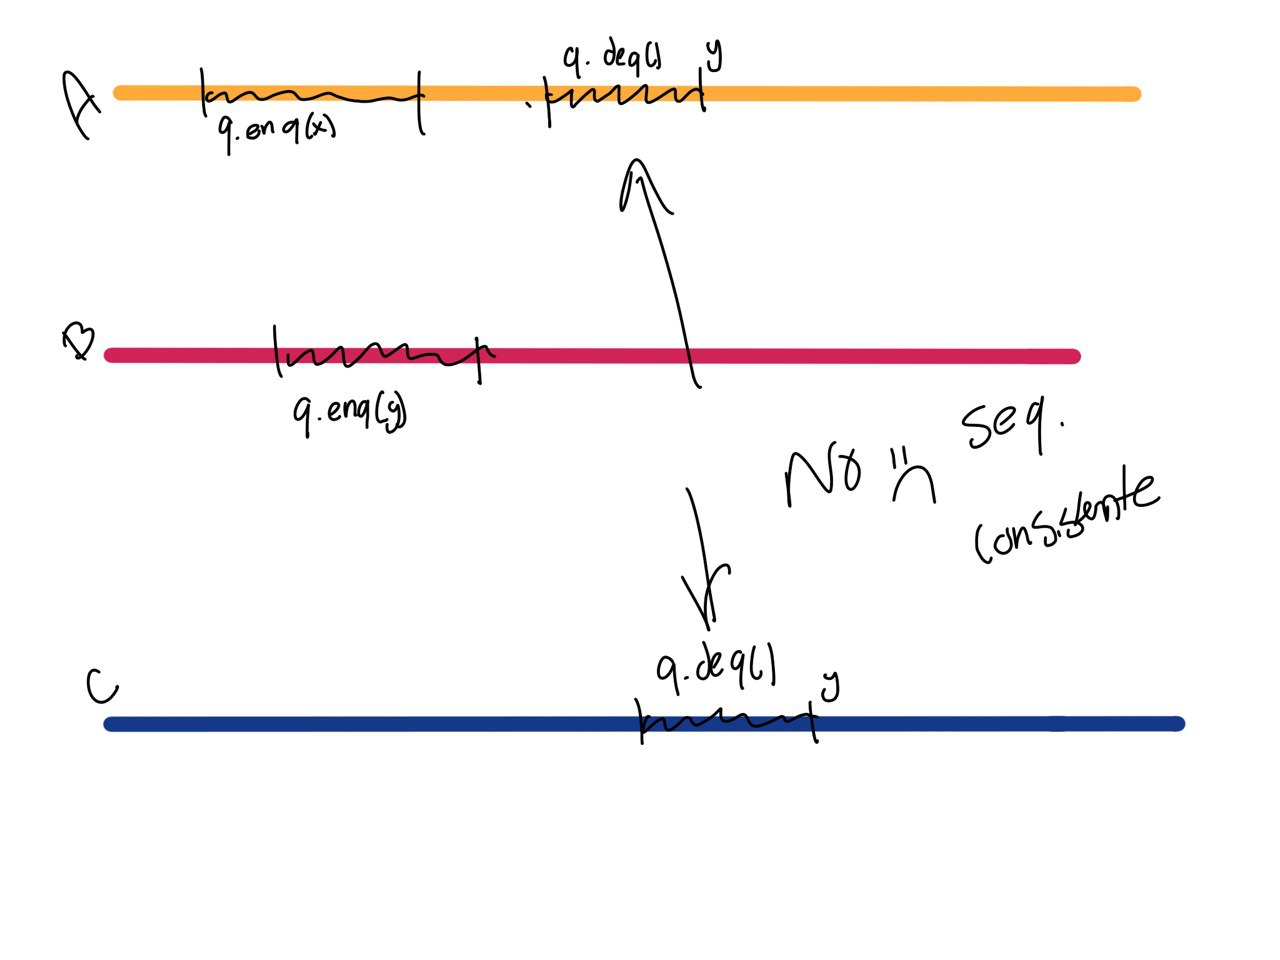
\includegraphics[width=0.3\textwidth]{Graphics/b_s}
              \caption{No es secuencialmente consistente, pues no importa el orden que pongamos
              non existen dos eventos de enq(y) que nos permitan explicar los 2 deq() que dan y}
            \end{figure}

            
            \begin{figure}[!h]
              \centering
              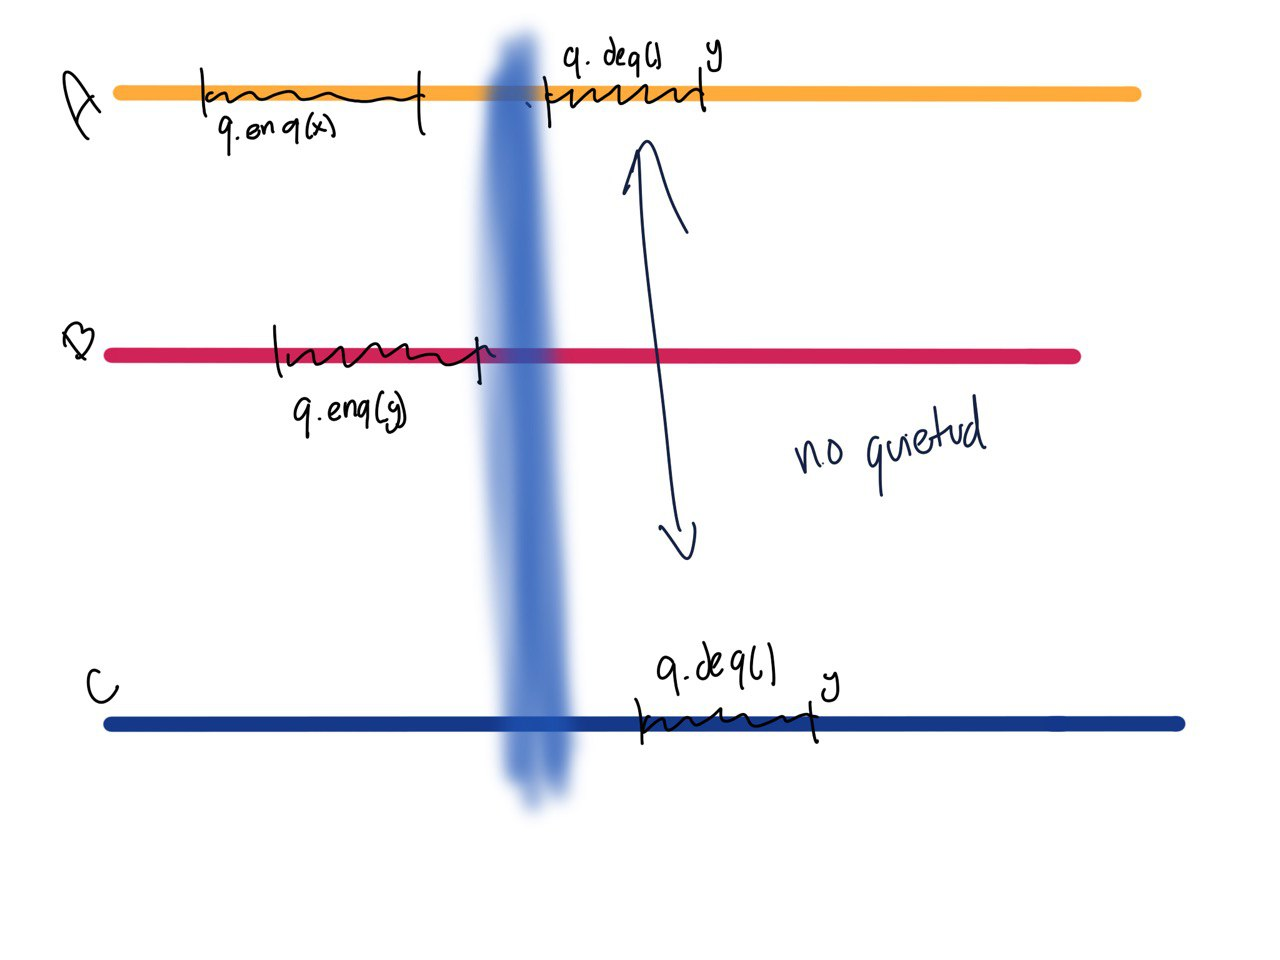
\includegraphics[width=0.3\textwidth]{Graphics/b_q}
              \caption{No hay consistencia de quietud, pues no importa el orden que pongamos
              non existen dos eventos de enq(y) que nos permitan explicar los 2 deq() que dan y }
            \end{figure}

            \begin{figure}[!h]
              \centering
              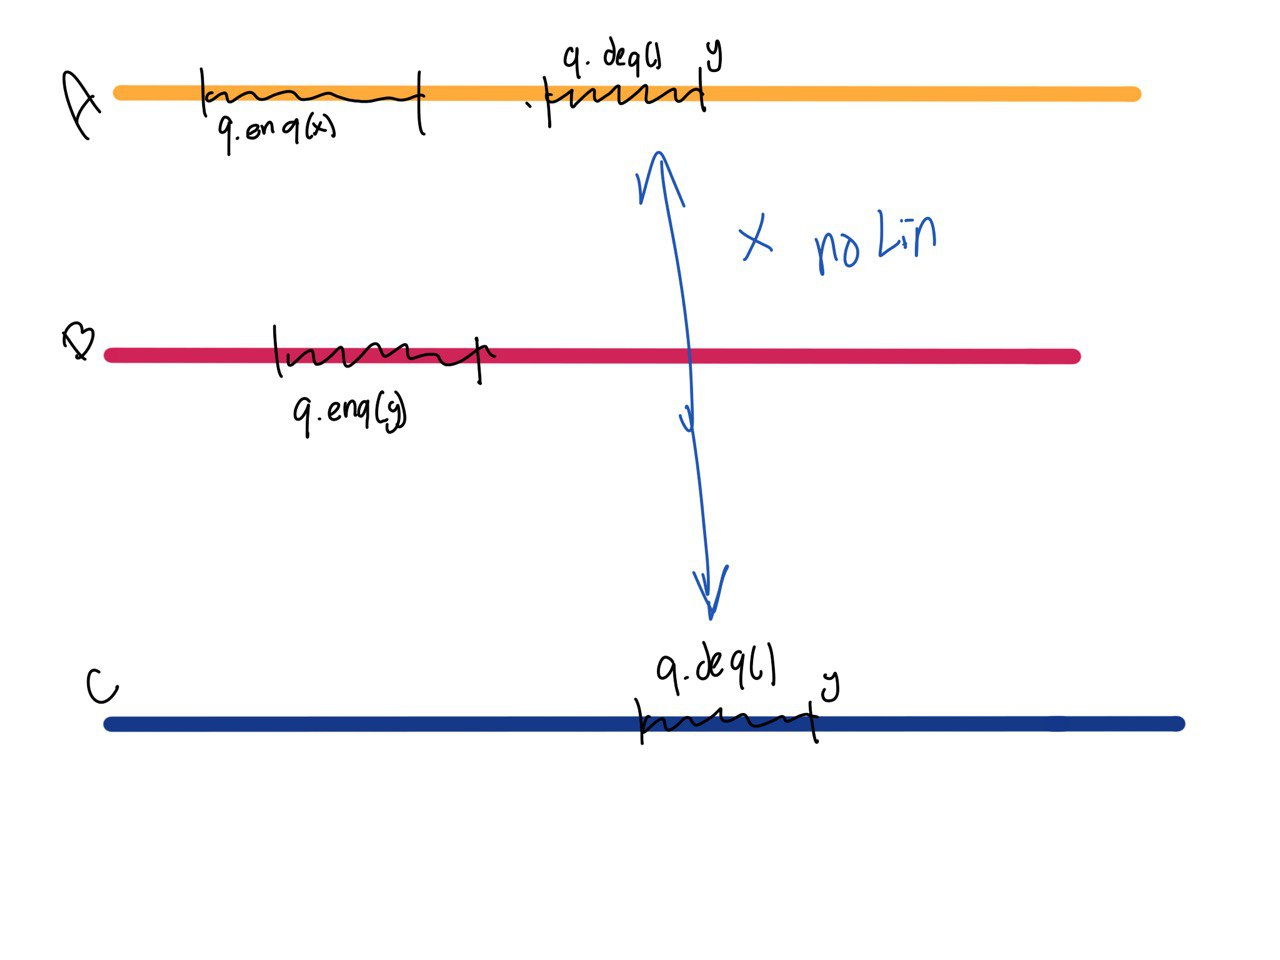
\includegraphics[width=0.3\textwidth]{Graphics/b_l}
              \caption{No es linearizable, pues no importa el orden que pongamos
              non existen dos eventos de enq(y) que nos permitan explicar los 2 deq() que dan y }
            \end{figure}

        }
        \clearpage
        \item{
        \begin{verbatim}
<A, s.push(10)>
<C, s.tryPop()>
<B, s.tryPop()>
<A, s:void>
<A, s.push(20)>
<B, s:10>
<A, s:void>
<C, s:emptyException>
        \end{verbatim}

        \begin{figure}[!h]
          \centering
          
\includegraphics[width=0.3\textwidth]{Graphics/c}
          \caption{El diagrama sería}
        \end{figure}

        
        \begin{figure}[!h]
          \centering
          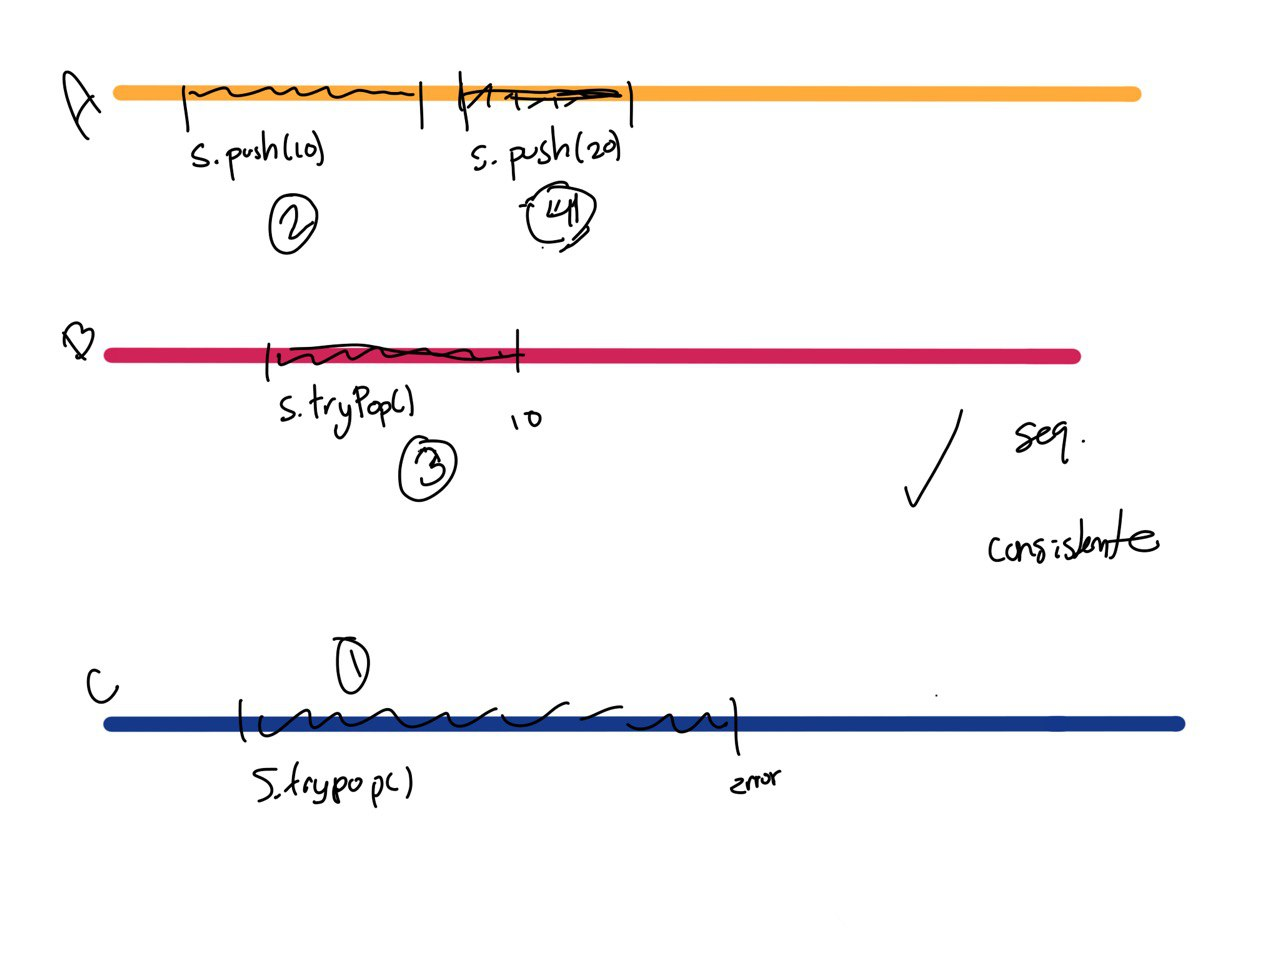
\includegraphics[width=0.3\textwidth]{Graphics/c_s}
          \caption{Secuencialmente consistente, pues podemos darle un orden a los eventos
          tal que el orden de los eventos dentro de cada hilo se mantiene y el orden
          resultante tiene sentido. }
        \end{figure}

        
        \begin{figure}[!h]
          \centering
          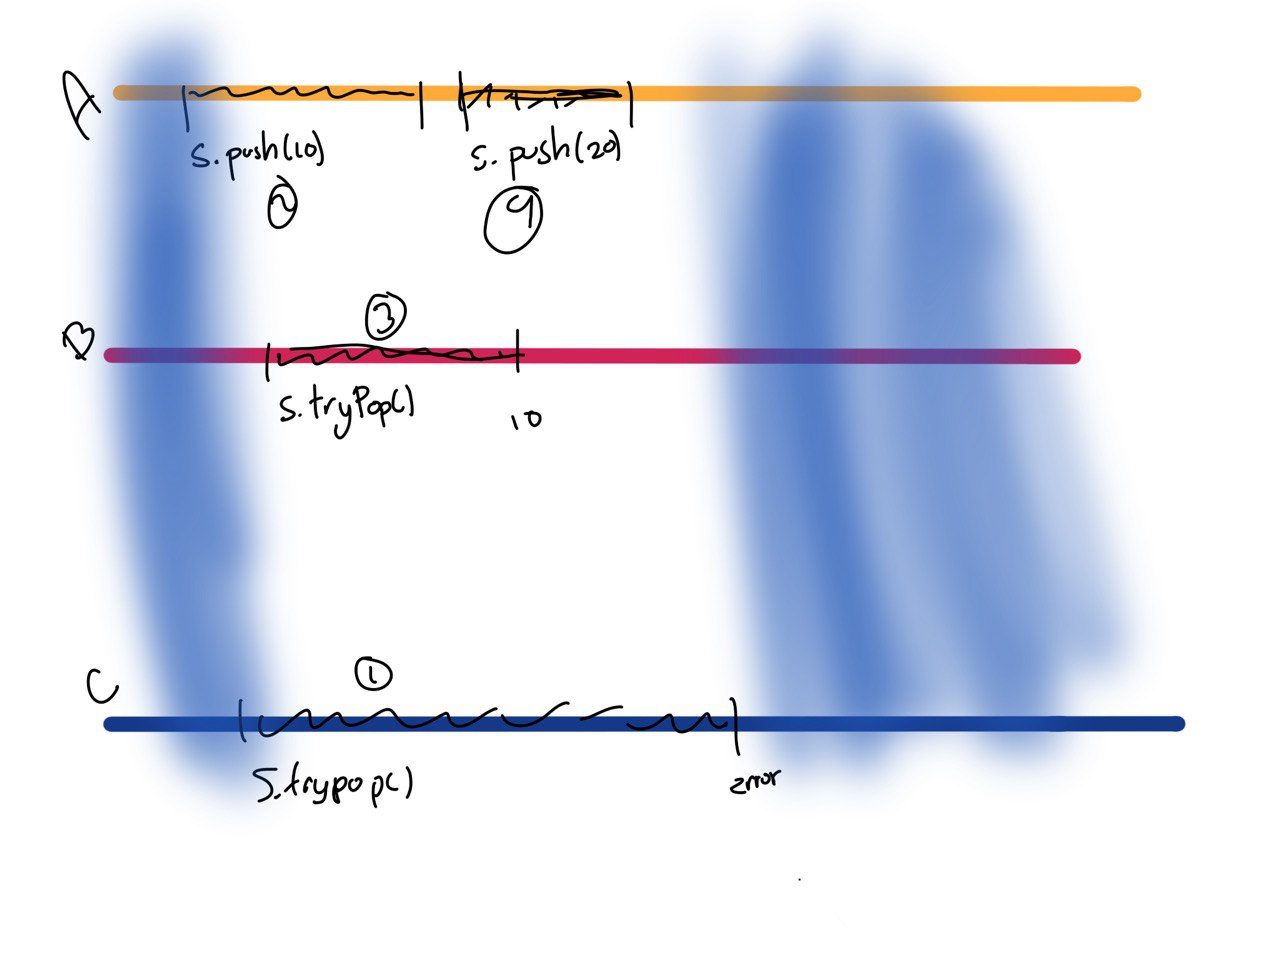
\includegraphics[width=0.3\textwidth]{Graphics/c_q}
          \caption{Consistencia de quietud, pues solo existe un espacio de quietud, y podemos
          dar un orden, el que mostramos por ejemplo, donde se respeta el orden de los eventos
          por bloques de quietud y el orden resultante tiene sentido, esto es mas facil pues
          todos los eventos ocurren en el mismo bloque. }
        \end{figure}

        \begin{figure}[!h]
          \centering
          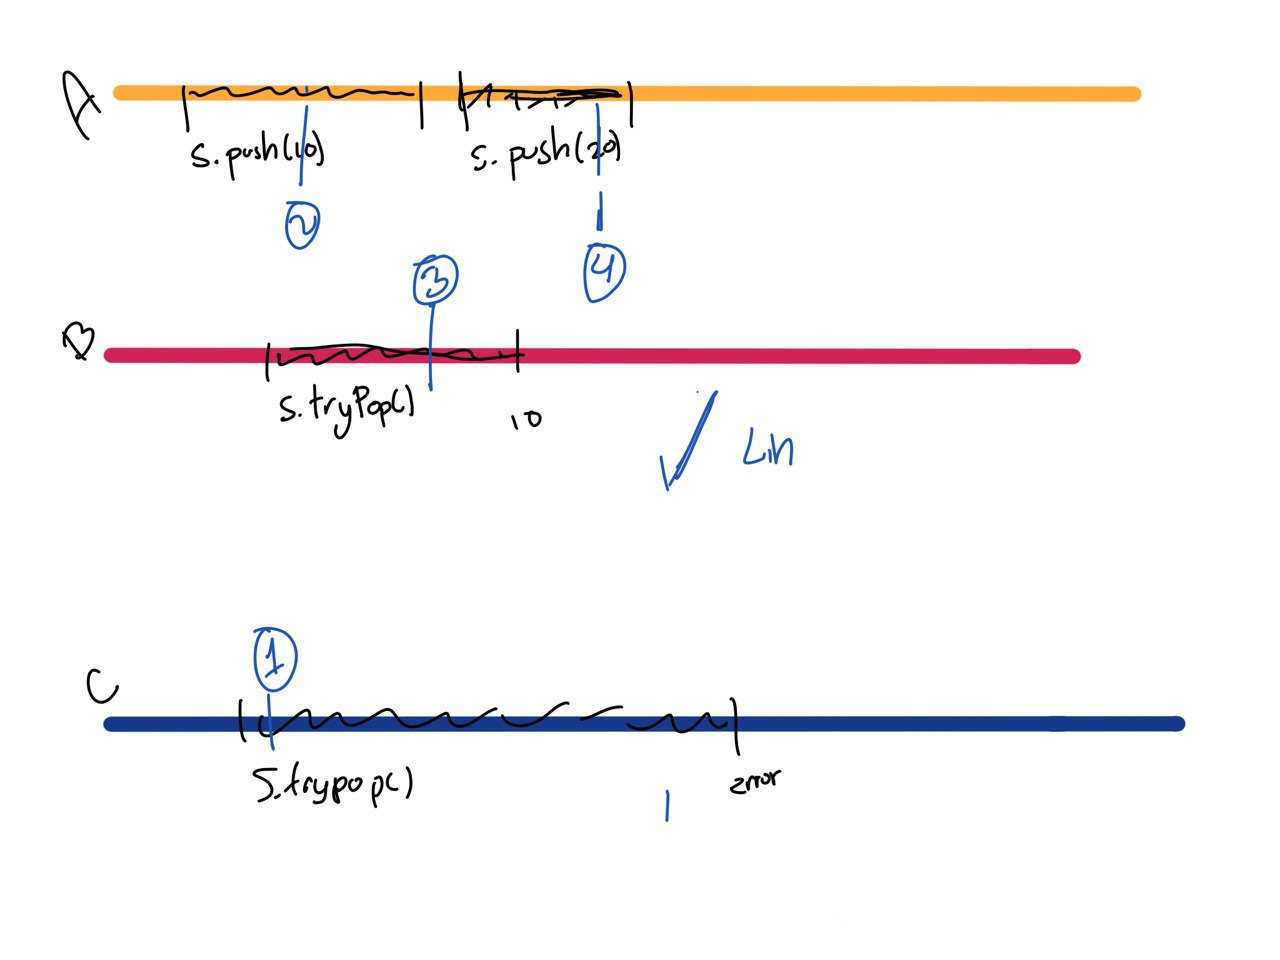
\includegraphics[width=0.3\textwidth]{Graphics/c_l}
          \caption{Linearizable, pues podemos dar un tiempo puntual para cada evento y con ello
          un orden resultante que tiene sentido. }
        \end{figure}

        }
    \end{enumerate}
    }

    \clearpage

    \item {\textbf{[1.0pt]} Da  un  ejemplo  de  una  ejecución  que  tenga  consistencia  de  quietud  pero  no secuencial; y otra que tenga consistencia secuencial pero no de quietud. Argumenta porque las ejecuciones no cumplen con cada propiedad
    
    \begin{figure}[!h]
      \centering
      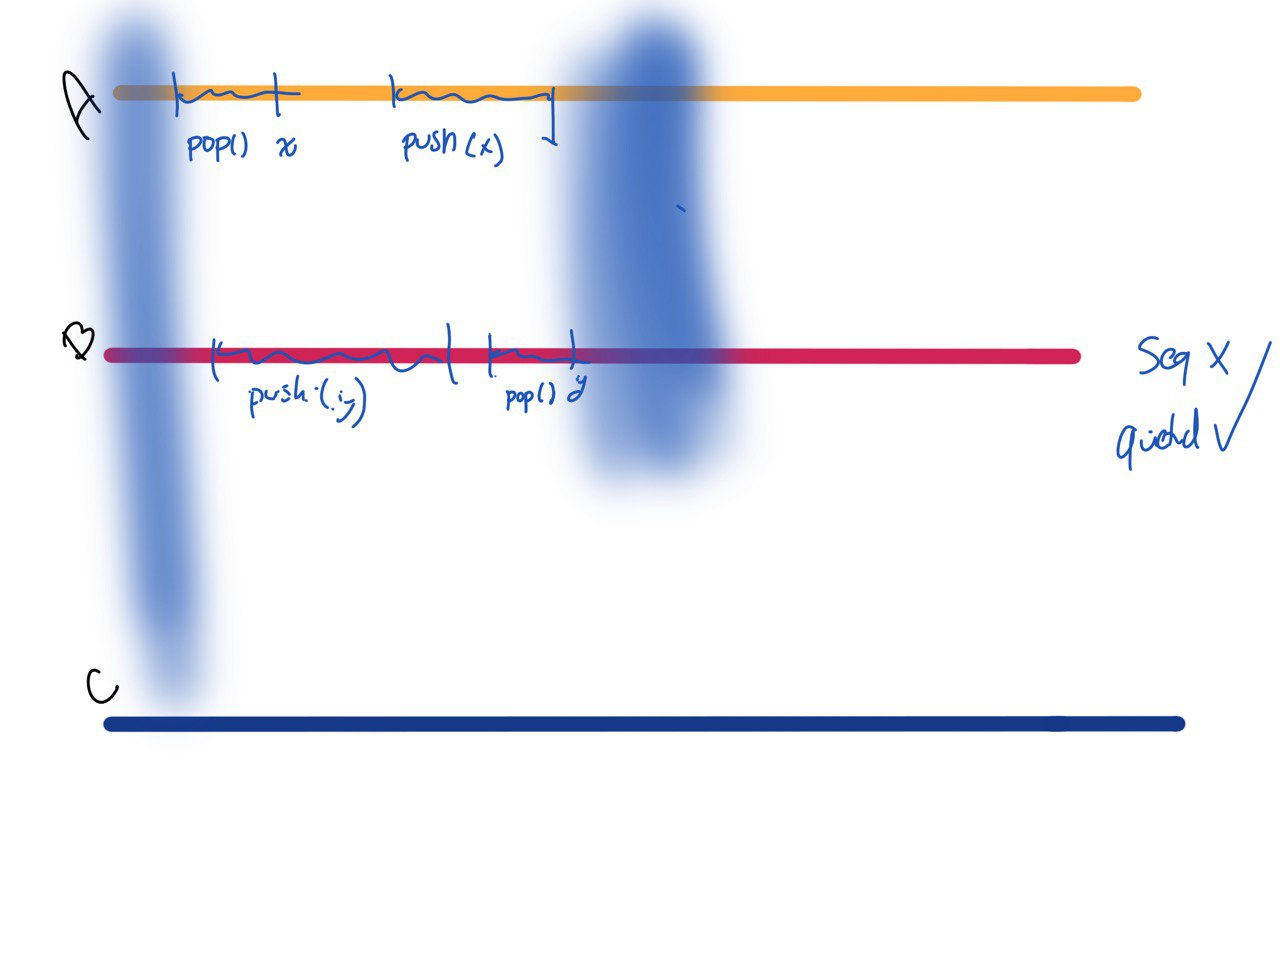
\includegraphics[width=0.7\textwidth]{Graphics/na}
      \caption{La idea es sencilla, es facil acomodar los eventos para mostrar la consistencia de quietud, 
      pues al estar en el mismo bloque podemos poner primero el push del hilo a, luego el pop del hilo a, luego el push del hilo b y
      luego el pop del hilo b, pero debido a que en la consistencia secuencial no podemos mover el order de los eventos de un mismo hilo es imposible lograr un dato de un pop que solo puede provenir de un push posterior}
    \end{figure}

    \begin{figure}[!h]
      \centering
      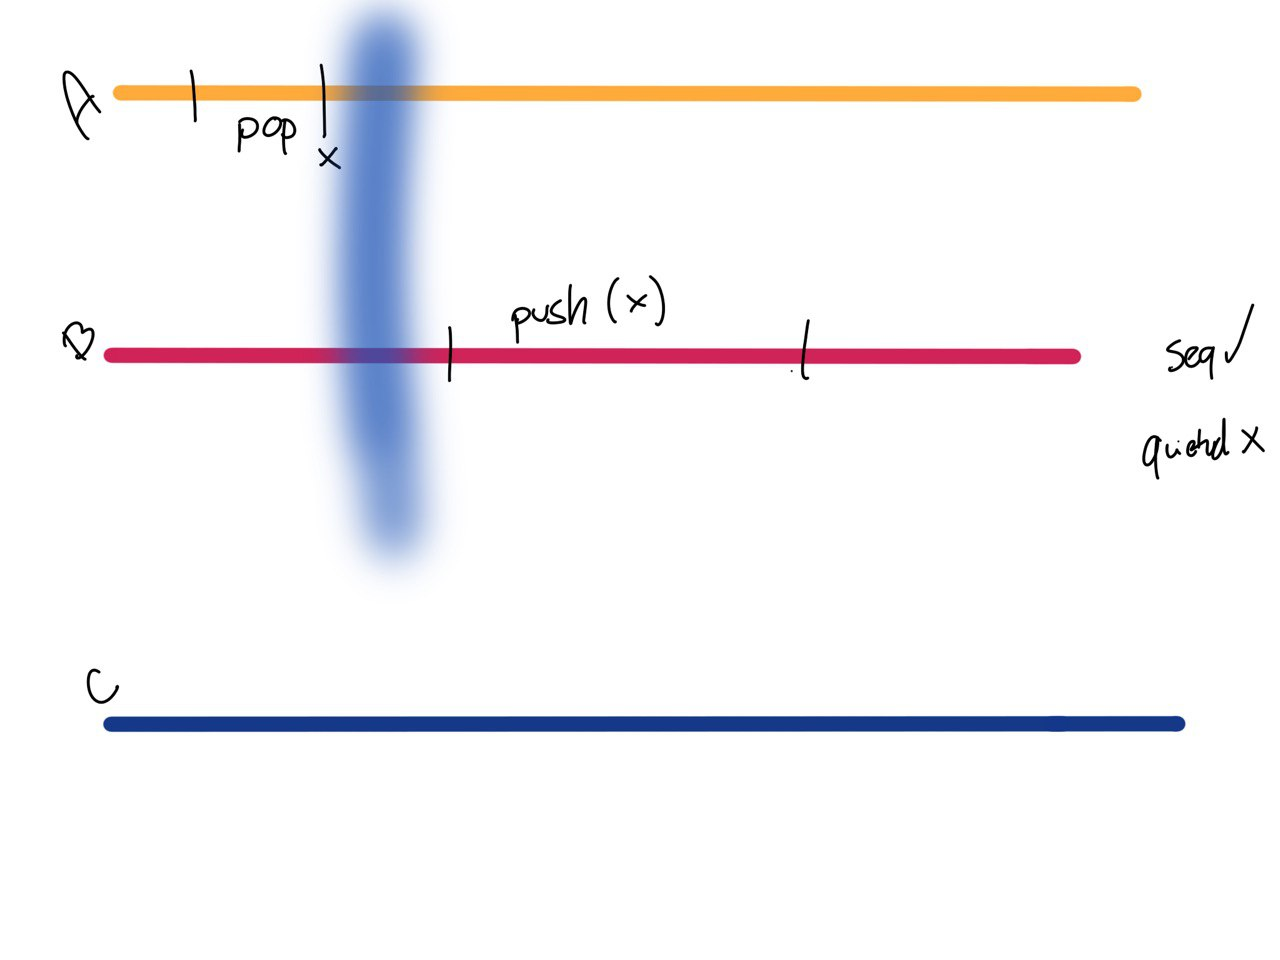
\includegraphics[width=0.7\textwidth]{Graphics/nb}
      \caption{La idea es poner un espacio de quietud que oblige a pensar en que primero se hizo un pop, lo cual es imposible, pero es trivial resolver el problema si buscamos consistencia secuencial, 
      pues podemos mover el order y decir que el evento del hilo b se ejecuto primero, y al final el hilo a}
    \end{figure}
    }
    \clearpage

    \item
    \textbf{[2.0pt]} 
    
    Demuestra que la siguiente implementación no es linearizable para más de 3 hilos:
    \begin{tcolorbox}
\begin{lstlisting}[language = JAVA]
public void enq(T x) {
  if (tail - head == capacity)
    throw FullException();
  items[tail % capacity] = x;
  tail++;
}

public T deq() {
  if (tail - head == 0)
    throw EmptyException();
  T x = items[head % capacity];
  head++;
  return x
}

\end{lstlisting}
\end{tcolorbox}






\end{enumerate}
\end{document}
